% v2 manuscript candidate (2026-09-04 revision after the multi-lens review). Every scientific number is a macro
% from numeric_insert_paper.tex (derived mechanically from the frozen scorer's numeric_insert.tex), tables_v2.tex
% (tools.paper_tables), descriptor_macros.tex (tools.paper_descriptors) or carried_audit.tex (record-279 audit
% values, carried, not re-estimated). Design constants (unit counts, corpus sizes) are typed and listed by
% tools.check_paper_numbers. Author metadata and the official ICASSP 2027 template remain pending.
\documentclass{article}
\usepackage{spconf,amsmath,graphicx,booktabs}
\InputIfFileExists{numeric_insert_paper.tex}{}{\PackageError{v2}{numeric_insert_paper.tex is absent}{run tools.tex_macros on runs/main/numeric_insert.tex}}
\InputIfFileExists{tables_v2.tex}{}{\PackageError{v2}{tables_v2.tex is absent}{run tools.paper_tables}}
\InputIfFileExists{carried_audit.tex}{}{\PackageError{v2}{carried_audit.tex is absent}{copy the record-279 S1 macros}}
\InputIfFileExists{descriptor_macros.tex}{}{\PackageError{v2}{descriptor_macros.tex is absent}{run tools.paper_descriptors}}
\title{WHERE DOES THE SPEAKER-OVERLAP PREMIUM IN SPEECH EMOTION RECOGNITION COME FROM?\\
A PREREGISTERED FACTORIAL, MECHANISM AND FINE-TUNING STUDY}
\name{AUTHOR METADATA REQUIRED BEFORE SUBMISSION}
\address{AFFILIATION AND EMAIL REQUIRED BEFORE SUBMISSION}
\begin{document}
\ninept
\maketitle

\begin{abstract}
Speaker-nonexclusive evaluation is common in public speech emotion recognition (SER) code: our earlier probability audit of \SOneFrameN{} repository lineages resolved \SOneYes{} of \SOneSampleN{} sampled lineages as permitting the same speaker on both sides of an active boundary, with \SOneUnknown{} unresolved [14].
Here we ask what that practice buys and why.
We call the out-of-fold UAR difference between a speaker-nonexclusive pipeline and a fully speaker-exclusive one its \emph{premium}.
In a preregistered one-shot program (4,943 registered units, frozen registry, code-independent verifier) we cross the outer test partition with the inner model-selection split, each random (R) or speaker-grouped (G), giving cells RR, RG, GR and GG (first letter outer, second inner), on RAVDESS, CREMA-D and a repetition-clean SUBESCO panel (SUBESCO-980), for three from-scratch models and three frozen self-supervised probes.
On SUBESCO-980 the premium RR$-$GG was \HNZeroOneMean{} points (95\% CI \HNZeroOneCILow{} to \HNZeroOneCIHigh; \HNZeroOneVerdict), decomposing into outer test leakage RG$-$GG of \HNZeroThreeMean{} and inner selection leakage RR$-$RG of \HNZeroFourMean{} points.
A matched-size speaker$\times$prompt checkerboard separates prompt overlap from cross-prompt speaker overlap on CREMA-D (\HNZeroFiveMean{} and \HNZeroSixMean{} points), and a size-matched 24- vs.\ 91-speaker contrast tests the speaker-count/density moderator (\HNOneZeroMean{} points, \HNOneZeroVerdict).
Under partial fine-tuning of WavLM-base+ the premium persists (RAVDESS \HRZeroNineMean, CREMA-D \HROneZeroMean, SUBESCO-980 \HROneOneMean{} points).
Verdicts follow the frozen claim map.
\end{abstract}

\begin{keywords}
speech emotion recognition, evaluation protocol, speaker independence, preregistration, data leakage
\end{keywords}

\section{Introduction}

SER systems are usually interpreted as generalizing to unseen speakers.
That interpretation requires speaker exclusivity at every active boundary: the outer test partition and any inner validation split used for checkpoint or hyperparameter selection.
Fold criteria are known to change SER scores [3]--[5], and our earlier probability audit of public SER code (locally frozen sampling and endpoint contracts, no public pre-outcome registration, outcome-visible revised lineage rule) found speaker-nonexclusivity risk in \SOneYes{} of \SOneSampleN{} sampled lineages (\SOneNo{} negative, \SOneUnknown{} unresolved; partial-identification interval \SOnePartialLowPct--\SOnePartialHighPct\%; finite-frame joint $\geq$95\% envelope \SOneEnvelopeLowPct--\SOneEnvelopeHighPct\%) [14].
What has not been measured is the structure of the resulting premium: how much comes from the outer boundary and how much from inner selection, whether it is driven by prompt overlap or by cross-prompt speaker identity, whether it depends on how many utterances each speaker contributes, and whether it survives fine-tuning of a modern self-supervised encoder.

This paper reports a preregistered one-shot program designed to answer those questions: the registry of 28 hypotheses, the claim map, every split table, the scorer and a code-independent verifier were frozen before any real-data fit (tag \texttt{SER26-prereg-1}; a second tag recorded only a timing probe).
The headline claims are C2, the premium and its outer/inner decomposition on SUBESCO-980, replicated on RAVDESS and CREMA-D; C3, the mechanism (prompt overlap, cross-prompt speaker overlap, sibling takes, speaker count/density) at matched training size; and C4, persistence of the premium under partial fine-tuning of WavLM-base+, with the change relative to a frozen same-regime comparator reported as an estimate; the audit prevalence (C1) is carried from [14].

\section{Relation to prior work}

SER evaluation has long distinguished speaker-dependent from speaker-independent settings [1], and splitting criteria change absolute scores and sometimes rankings [2]--[5]; reproducibility [6], motivation--dataset alignment [7], standardized speaker-independent partitions [8], [9] and non-emotion shortcuts [10] have each been studied.
None of this work separates the outer and inner boundaries, holds training size constant while toggling speaker and prompt overlap, or estimates against a frozen same-regime comparator how much fine-tuning changes the premium; our contribution is the design that does, executed once under a public preregistration.

\section{Preregistered design}

\subsection{Corpora, hygiene and corpus levels}
RAVDESS speech (24 speakers, 8 classes) [11], CREMA-D (91 speakers, 6 classes) [12] and SUBESCO (20 Bangla speakers, 10 prompts, 7 emotions, 5 takes) [13] were byte-manifested.
Preregistered hygiene removed exact-duplicate groups with conflicting labels (CREMA-D, 3 groups), kept the lexically first path of single-label duplicates (RAVDESS 1, SUBESCO 2) and one registered unusable file (CREMA-D), giving 1,439 / 7,435 / 6,998 utterances.
We call each evaluated corpus or panel a \emph{corpus level}.
The three \emph{primary} levels enter the confirmatory families: RAVDESS, CREMA-D and SUBESCO-980, a pinned repetition-clean panel (7 prompts $\times$ one take per speaker--prompt--emotion combination, 980 utterances) on which sibling takes cannot leak.
Secondary levels are SUBESCO-full, three SUBESCO panels (1,400 combinations $\times$ 1 take; 700 $\times$ 1; 700 $\times$ 2), five stratified 24-speaker CREMA-D draws and five utterance-matched 91-speaker draws (CNN, ResNet-SE and the three probes, RR and GG only, two replicates per CREMA-D draw and three otherwise; the take-grouped SUBESCO-full cell is CNN only).

\subsection{Protocol factorial}
Every primary level is evaluated in four cells that cross the outer and inner boundaries: outer random (R, stratified five-fold) or speaker-grouped (G) partitions, and inner fit/validation splits of the outer training fold that are random (R) or speaker-grouped (G); RR is the speaker-nonexclusive pipeline and GG the speaker-exclusive one, RG$-$GG isolates outer test leakage, RR$-$RG inner selection leakage, and GR$-$GG the cost of grouping the inner split when the test is already exclusive.
Three replicates (partition draw and training seed indexed together) are run for three from-scratch models (CNN, ResNet-SE, Transformer: the P1 architectures and optimization contract of [14], AdamW with cosine annealing, class-balanced cross-entropy, 100 epochs, patience 15, checkpoint on validation loss) and three frozen probes (early-stopped linear heads on fit-fold-standardized time means of the final hidden state of HuBERT-base, WavLM-base+ and wav2vec2-base at 16 kHz).
Scratch inputs are the P1 front end: 22.05 kHz mono, 30 dB trim, 64 log-mel bins, 128 frames, per-utterance z-score, with train-only SpecAugment (two time and two frequency masks plus Gaussian noise).
A draw$\times$seed crossing (CNN, RAVDESS and SUBESCO-980) separates partition and training randomness, and the four P1 outer partitions with their seed-specific inner splits reconcile with [14].

\subsection{Mechanism block}
\begingroup\sloppy
On CREMA-D (12 sentences) and SUBESCO-full (10 prompts) speakers and prompts are split into five groups each; a speaker$\times$prompt checkerboard fixes the test set (speaker group $i$ $\times$ prompt group $j$, one item per speaker--sentence--label combination; remaining takes or intensity variants are held out of training) and draws four training conditions from the legal pools with identical training size ($\approx$3,440 / 3,359 fit utterances), class stratification and inner rule: \emph{none} (speaker- and prompt-exclusive), \emph{spk} (test speakers' other prompts), \emph{prm} (other speakers' test prompts) and \emph{both}; SUBESCO-full adds \emph{both+sib} (sibling takes of the test items), and both corpora add two complementary half-exposure conditions (h1, h2) in which a hash-selected half of the test speakers contributes its other-prompt items.
Two prompt-group rotations over the five speaker-group folds and two replicates give 20 fits per condition and model (CNN, ResNet-SE).
Absolute UAR in this block is not comparable to the factorial because training sets are subsampled to the smallest legal pool.\par\endgroup

\subsection{Fine-tuning, HPO and Ridge supplements}
WavLM-base+ is partially fine-tuned (top four transformer layers, mean pool, linear head; AdamW, encoder/head learning rates $5\times10^{-5}$/$10^{-3}$, weight decay $10^{-2}$, batch 16, fp16, constant learning rate, class-balanced cross-entropy, 15 epochs, patience 3 on validation loss; random 3-s training crops, first 10 s at evaluation) and compared with a frozen same-regime comparator: identical head, folds, seeds and epoch budget, encoder frozen but in training mode (dropout active), unstandardized mean features.
Both run on the first RR and GG partition draw of each primary level with two seeds (the conditional CREMA-D second seed was run).
An HPO arm searches eight ResNet-SE configurations under a fixed speaker-exclusive outer test with random (GR) or grouped (GG) inner validation, plus an RR descriptor cell whose outer test is speaker-overlapping, on CREMA-D (primary) and RAVDESS (secondary); a CPU Ridge arm supplies head-effect and LOSO-equivalence supplements on the same partitions, and a 20-draw $\times$ 13-state Ridge layer sweep (54,600 fits) feeds descriptors D12--D13 only.

\subsection{Statistics, freeze, verification and execution}
The unit of inference is the speaker; per-speaker out-of-fold UAR is averaged over replicates and over the models of a group before differencing.
Each registered hypothesis reports the mean speaker-paired difference, a 10,000-replicate whole-speaker percentile bootstrap CI and a two-sided Wilcoxon test (an exact sign test is added as a sensitivity when more than 20\% of speakers tie; the Holm family always uses the Wilcoxon $p$), Holm-adjusted within claim-wise families (N-decomp 4, N-mech 4, N-supp 2, R 11, T 2); hypotheses whose simulated Holm power was below 0.5 (N07, N08, N11--N13) were demoted a priori to estimates and are reported with intervals only.
Equivalence claims use TOST with preregistered margins.
Claim verdicts are computed structurally from the frozen claim map, whose forbidden readings (prevalence$\times$effect products, ``uses voiceprint'', dose curves, language causality) we observe.
A verifier written from the specification alone, sharing no code with the scorer but authored by the same agent in a separate pass, agreed with the scorer on every hypothesis, claim and on descriptors D01--D03, D05, D06, D09 and D14 to within $10^{-12}$ on a synthetic full run and on the real results; a 20-case battery (18 injected faults, each detected, plus null-world and sign-flip checks) behaved as specified before the freeze; a post-hoc key map reconciled D04, D07 and D08 (\DReconcileItems{} values, max difference \DReconcileMaxDiff).
Units ran in six disjoint parallel queues with arms overlapping in time (order-invariant by per-unit seeding); deviation entries 1--2 record the budget outcome.

\section{Results}

\subsection{Premium and its decomposition (C2)}
Table~1 gives the four cells per level and model and Fig.~\ref{fig:contrasts} the scratch-group contrasts.
On SUBESCO-980 the scratch premium RR$-$GG was \HNZeroOneMean{} points (95\% CI \HNZeroOneCILow{} to \HNZeroOneCIHigh, $n=\HNZeroOneN$, Holm $p$ $\HNZeroOnePHolm$; \HNZeroOneVerdict); the probe premium was \HNZeroTwoMean{} points (\HNZeroTwoCILow{} to \HNZeroTwoCIHigh; \HNZeroTwoVerdict).
Outer test leakage RG$-$GG contributed \HNZeroThreeMean{} points (\HNZeroThreeCILow{} to \HNZeroThreeCIHigh; \HNZeroThreeVerdict) and inner selection leakage RR$-$RG \HNZeroFourMean{} points (\HNZeroFourCILow{} to \HNZeroFourCIHigh; \HNZeroFourVerdict); C2a is \ClaimCTwoa{} and C2b \ClaimCTwob.
The same-implementation replications on RAVDESS (R01--R03: \HRZeroOneMean, \HRZeroTwoMean, \HRZeroThreeMean{} points) and CREMA-D (R04--R06: \HRZeroFourMean, \HRZeroFiveMean, \HRZeroSixMean) and the probe premia (R07 \HRZeroSevenMean{} [\HRZeroSevenCILow, \HRZeroSevenCIHigh]; R08 \HRZeroEightMean{} [\HRZeroEightCILow, \HRZeroEightCIHigh]) give C2-rep \ClaimCTworep.

\begin{table*}[t]
\centering\scriptsize
\caption{Protocol factorial: mean over speakers of the replicate-averaged per-speaker out-of-fold UAR (\%) in the four cells and the three speaker-paired contrasts (points). RR = random outer and inner; RG = random outer, grouped inner; GR = grouped outer, random inner; GG = grouped outer and inner. Contrasts use unrounded means (may differ from rounded-cell differences by 0.01).}
\TabFactorial
\end{table*}

\subsection{Mechanism (C3)}
Table~2 gives the matched-size conditions.
On CREMA-D, prompt overlap alone (prm$-$none) added \HNZeroFiveMean{} points (\HNZeroFiveCILow{} to \HNZeroFiveCIHigh; \HNZeroFiveVerdict) and cross-prompt speaker overlap alone (spk$-$none) \HNZeroSixMean{} points (\HNZeroSixCILow{} to \HNZeroSixCIHigh; \HNZeroSixVerdict).
On SUBESCO-full the a-priori estimates were \HNZeroSevenMean{} [\HNZeroSevenCILow, \HNZeroSevenCIHigh] and \HNZeroEightMean{} [\HNZeroEightCILow, \HNZeroEightCIHigh] points (not tested).
Sibling takes added \HNZeroNineMean{} points at matched size (\HNZeroNineCILow{} to \HNZeroNineCIHigh; \HNZeroNineVerdict).
At matched utterance count, the 24-speaker panels inflated more than the utterance-matched 91-speaker panels by \HNOneZeroMean{} points (\HNOneZeroCILow{} to \HNOneZeroCIHigh; \HNOneZeroVerdict).
Claims: C3a \ClaimCThreea, C3b \ClaimCThreeb, C3c \ClaimCThreec, C3d \ClaimCThreed.

\begin{table*}[t]
\centering\scriptsize
\caption{Mechanism block (UAR \%, mean over speakers; 20 fits per condition and model). none = speaker- and prompt-exclusive training; spk / prm = test speakers' other prompts / other speakers' test prompts added; both = both; both+sib = both plus sibling takes (SUBESCO-full only); exposed / unexposed half = a speaker's UAR in the half-exposure condition in which it is / is not exposed (as in T02, D06).}
\TabMech
\end{table*}

\subsection{Modern pipeline (C4)}
Table~3 gives the WavLM-base+ cells.
The fine-tuned premium RR$-$GG was \HRZeroNineMean{} points on RAVDESS (\HRZeroNineCILow{} to \HRZeroNineCIHigh; \HRZeroNineVerdict), \HROneZeroMean{} on CREMA-D (\HROneZeroCILow{} to \HROneZeroCIHigh; \HROneZeroVerdict) and \HROneOneMean{} on SUBESCO-980 (\HROneOneCILow{} to \HROneOneCIHigh; \HROneOneVerdict); C4a is \ClaimCFoura.
Relative to the frozen same-regime comparator, fine-tuning changed the premium by \HNOneOneMean{} [\HNOneOneCILow, \HNOneOneCIHigh], \HNOneTwoMean{} [\HNOneTwoCILow, \HNOneTwoCIHigh] and \HNOneThreeMean{} [\HNOneThreeCILow, \HNOneThreeCIHigh] points (a-priori estimates; C4b reported without a verdict).

\begin{table}[t]
\centering\scriptsize
\caption{WavLM-base+ partial fine-tuning vs.\ the frozen same-regime comparator (UAR \%, first partition draw, seeds averaged; frozen rows are not the Table~1 probe regime; contrasts use unrounded means).}
\TabFT
\end{table}

\begin{figure}[t]
\centering
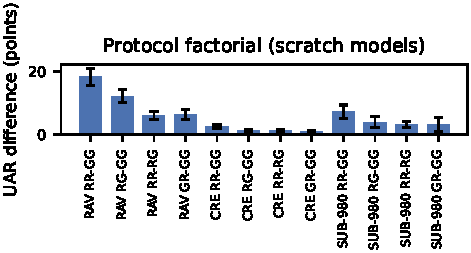
\includegraphics[width=\columnwidth]{figure_v2.pdf}
\caption{Protocol-factorial contrasts of the scratch group (UAR points, 95\% whole-speaker bootstrap intervals); RAV = RAVDESS, CRE = CREMA-D, SUB-980 = SUBESCO-980; GR$-$GG is descriptor D01.}
\label{fig:contrasts}
\end{figure}

\subsection{Supplements and descriptors}
Descriptor intervals are 95\% whole-speaker bootstrap intervals without inference.
On CREMA-D (ResNet-SE), hyperparameter selection on a speaker-overlapping inner validation was more optimistic than on a grouped one by \HNOneFourMean{} points (\HNOneFourCILow{} to \HNOneFourCIHigh; S1 \ClaimSOne); the honest outer-test difference-in-differences was \DNine{} points (\DNineLo{} to \DNineHi; D09).
The RR$_{\mathrm{hpo}}$ cell, whose outer test is random, reported \DEightRRminusGG{} points (\DEightRRminusGGLo{} to \DEightRRminusGGHi) more than GG$_{\mathrm{hpo}}$ on CREMA-D and \DEightRRminusGGRav{} (\DEightRRminusGGRavLo{} to \DEightRRminusGGRavHi) on RAVDESS; selecting a configuration on the outer test would have added \DEightOptimismGR{}--\DEightOptimismGG{} points across the three CREMA-D cells (D08).
On RAVDESS, the outer-boundary premium was \HNOneFiveMean{} points (\HNOneFiveCILow{} to \HNOneFiveCIHigh) larger for a Ridge head than for the linear probes on identical partitions (S2 \ClaimSTwo).
On CREMA-D frozen features, size-matched LOSO and five-fold grouping were equivalent within $\pm$1 point (T01, mean $\HTZeroOneMean$, TOST Holm $p$ $\HTZeroOnePHolm$; S3 \ClaimSThree); descriptively, on RAVDESS CNN full LOSO exceeded five-fold grouping by \DFifteenLOSOminusGFive{} points (\DFifteenLOSOminusGFiveLo{} to \DFifteenLOSOminusGFiveHi) and size-matched LOSO by \DFifteenSUBminusGFive{} (\DFifteenSUBminusGFiveLo{} to \DFifteenSUBminusGFiveHi; D15).
On CREMA-D, spillover to unexposed co-fold speakers was absent within $\pm$1.5 points (T02, mean $\HTZeroTwoMean$, TOST Holm $p$ $\HTZeroTwoPHolm$; S4 \ClaimSFour); the half-exposure gain was \DSixShareCre{} (CREMA-D) and \DSixShareSub{} (SUBESCO-full) of the full speaker-overlap gain, and the speaker$\times$prompt interaction was \DSixInterCre{} (\DSixInterCreLo{} to \DSixInterCreHi) and \DSixInterSub{} (\DSixInterSubLo{} to \DSixInterSubHi) points (D06).
The GR$-$GG allocation cost was \DOneScratchRav, \DOneScratchCre{} and \DOneScratchSub{} points on RAVDESS, CREMA-D and SUBESCO-980 (D01), every model had a positive RR$-$GG sign on every primary level (D02), and RAVDESS inflated more than CREMA-D by \DThreeRavCre{} points (\DThreeRavCreLo{} to \DThreeRavCreHi) and more than SUBESCO-980 by \DThreeRavSub{} (\DThreeRavSubLo{} to \DThreeRavSubHi; D03).
On SUBESCO, a second take per combination added \DFourTakes{} points (\DFourTakesLo{} to \DFourTakesHi) whereas doubling combinations at one take added \DFourCells{} (\DFourCellsLo{} to \DFourCellsHi; D04); random splitting of the full corpus exceeded take-grouped splitting by \DFive{} points (\DFiveLo{} to \DFiveHi; D05).
The Ridge premium was direction-stable (at least 18 of 20 draws positive, 5th percentile above zero) for \DThirteenStable{} of \DThirteenTotal{} encoder$\times$level combinations (D13), and its Spearman correlation with state index was negative in \DTwelveNegRho{} of \DTwelveTotal{} combinations (median $\rho=\DTwelveMedianRho$; D12).
On the four P1 outer partitions, pooled UAR reconciled with the 2026 rows within about 1.2 UAR (D16); draw and seed variance components (D14) are in the repository.
Speaker-identity probes on the held-out panels gave RR$-$GG differences in above-chance speaker recall of $\DTenCtrlRavCnn$, $\DTenCtrlCreCnn$ and $\DTenCtrlSubCnn$ points (CNN) and $\DTenFtRav$, $\DTenFtCre$ and $\DTenFtSub$ (fine-tuned WavLM), positive in \DTenPositive{} of \DTenTotal{} checkpoint families (D10); under RR the cosine-nearest training item of a RAVDESS CNN test item was a same-speaker item for \DElevenCtrlRavCnnRRSamespeaker\% and a sibling take for \DElevenCtrlRavCnnRRSibling\% of test items, against 0\% under GG (D11).

\section{Discussion}
All 23 confirmatory hypotheses were supported after Holm correction, including both equivalence tests.
First, the premium is a whole-pipeline property: on SUBESCO-980 roughly half of it is outer test leakage and half inner selection leakage, and the inner component is substantial on RAVDESS and CREMA-D too, so grouping only the final test removes only part of the inflation.
Second, at matched training size both prompt overlap and cross-prompt speaker overlap inflate scores on CREMA-D, where prompt overlap was the larger tested term; on SUBESCO-full the untested estimates point the other way, and no between-corpus contrast was registered.
Sibling takes add a further increment and, at matched utterance count, fewer and denser speakers inflate more; the interaction terms (D06) and T02 are consistent with an item-level, roughly additive effect, a descriptive reading rather than a tested mechanism.
Third, the premium is not a from-scratch artifact: frozen probes show it on every primary level, it is largest in the early encoder layers (D12), and partial fine-tuning of WavLM-base+ reproduces it on all three corpora; descriptively, RR did not yield a consistently more speaker-identifiable representation (D10) but did change the training neighborhood of the test items (D11).
These results license statements about specified corpora, protocols and pipelines, not a universal correction factor, a mediation share, or the claim that a classifier ``used voiceprints''.

\section{Limitations}
Three acted corpora, one implementation, one preregistered split generator; the mechanism block subsamples training sets and its absolute scores are not comparable to the factorial.
N07, N08 and N11--N13 were demoted a priori by simulated power, so C4b is an estimation claim; independently, the frozen same-regime comparator reached low absolute UAR (Table~3) and its best checkpoint was the last epoch in \DFtFrozenBestLast{} of \DFtFrozenTotal{} fits (fine-tuned mean best epoch \DFtFtMeanBest), so the shared epoch budget truncates the comparator and the re-exposure estimates are bounded by a weak though regime-matched baseline.
Measured GPU time of the from-scratch units was two to three times the frozen cost model (CPU-bound augmentation loop); three arm caps were exceeded in measured hours while the program total (about 43 h) stayed under the 50 h cap, and no unit was truncated (deviation entries 1--2).
In the preregistered retrain check, \DRetrainIdentical{} of \DRetrainTotal{} re-run units reproduced their predictions byte for byte; the exception, an fp16 WavLM comparator unit (label agreement \DRetrainAgree\%, fold UAR \DRetrainUarMain{} vs.\ \DRetrainUarCheck), shows the fine-tuning arm is reproducible to sub-point but not bitwise precision.
The audit prevalence (C1) is carried from [14]; the program's audit arm (G5) was not executed because it needs a second human rater.

\section{Conclusion and reproducibility}
The speaker-overlap premium is a whole-pipeline effect, split between the outer test boundary and inner model selection, fed by prompt overlap, cross-prompt speaker overlap, sibling takes and speaker density at matched training size, and persistent under partial fine-tuning of WavLM-base+; when unseen-speaker generalization is the target, both boundaries must be speaker-exclusive and reported numbers should say which were.
All artifacts (including the complete registry table) are in the repository at tags \texttt{SER26-prereg-1}/\texttt{-2} and the execution branch; every number above is a generated macro (hypotheses, claims and D01--D09/D14 replayed by the verifier; D10--D13, D15, D16 from descriptor tools outside the frozen scorer; C1 carried from [14]; design constants typed and checked).
Claude (Anthropic) implemented and executed the program and drafted this text; Codex (OpenAI) reviewed the design; neither is an author, and the human authors must inspect the evidence and revise the text before submission.

\clearpage
\begin{thebibliography}{14}
\bibitem{schuller2009challenge} B. W. Schuller, S. Steidl, and A. Batliner, ``The INTERSPEECH 2009 Emotion Challenge,'' in \emph{Proc. Interspeech}, pp. 312--315, 2009.
\bibitem{pepino2020fusion} L. Pepino, P. Riera, L. Ferrer, and A. Gravano, ``Fusion approaches for emotion recognition from speech using acoustic and text-based features,'' in \emph{Proc. ICASSP}, pp. 6484--6488, 2020.
\bibitem{atmaja2021splitting} B. T. Atmaja and A. Sasou, ``Effect of different splitting criteria on the performance of speech emotion recognition,'' in \emph{Proc. TENCON}, pp. 760--764, 2021.
\bibitem{zielonka2022recognition} M. Zielonka et al., ``Recognition of emotions in speech using convolutional neural networks on different datasets,'' \emph{Electronics}, vol. 11, no. 22, Art. 3831, 2022.
\bibitem{ibrahim2026multimodal} E. Ibrahim, M. E. Ghoraba, and A. E. Ghoraba, ``Multimodal emotion recognition using hybrid deep feature fusion under speaker-independent evaluation,'' \emph{Scientific Reports}, vol. 16, Art. 19584, 2026.
\bibitem{antoniou2023designing} N. Antoniou, A. Katsamanis, T. Giannakopoulos, and S. Narayanan, ``Designing and evaluating speech emotion recognition systems: A reality check case study with IEMOCAP,'' in \emph{Proc. ICASSP}, pp. 1--5, 2023.
\bibitem{wong2026unrequited} T. Wong, Z. Talat, H. Aldarmaki, and A. Field, ``Unrequited Emotions: Investigating the Gaps in Motivation and Practice in Speech Emotion Recognition Research,'' arXiv:2604.25776, 2026.
\bibitem{scheidwasserclow2022serab} N. Scheidwasser-Clow, M. Kegler, P. Beckmann, and M. Cernak, ``SERAB: A multi-lingual benchmark for speech emotion recognition,'' in \emph{Proc. ICASSP}, pp. 7697--7701, 2022.
\bibitem{wu2024openemotion} H. Wu et al., ``Open-Emotion: A reproducible EMO-SUPERB for speech emotion recognition systems,'' in \emph{Proc. IEEE SLT}, pp. 510--517, 2024.
\bibitem{meyer2018classifiers} P. Meyer, E. Buschermohle, and T. Fingscheidt, ``What do classifiers actually learn? A case study on emotion recognition datasets,'' in \emph{Proc. Interspeech}, pp. 262--266, 2018.
\bibitem{livingstone2018ravdess} S. R. Livingstone and F. A. Russo, ``The Ryerson Audio-Visual Database of Emotional Speech and Song (RAVDESS),'' \emph{PLOS ONE}, vol. 13, no. 5, Art. e0196391, 2018.
\bibitem{cao2014cremad} H. Cao, D. G. Cooper, M. K. Keutmann, R. C. Gur, A. Nenkova, and R. Verma, ``CREMA-D: Crowd-sourced emotional multimodal actors dataset,'' \emph{IEEE Trans. Affect. Comput.}, vol. 5, no. 4, pp. 377--390, 2014.
\bibitem{sultana2021subesco} S. Sultana, M. S. Rahman, M. R. Selim, and M. Z. Iqbal, ``SUST Bangla Emotional Speech Corpus (SUBESCO): An audio-only emotional speech corpus for Bangla,'' \emph{PLOS ONE}, vol. 16, no. 4, Art. e0250173, 2021.
\bibitem{ours2026audit} [AUTHORS], ``Speaker-nonexclusivity risk in public SER code: a probability audit and controlled study of protocol effects,'' manuscript, 2026; repository tag \texttt{icassp2027-complete-2026-08-30} (release pending).
\end{thebibliography}

\end{document}
